\documentclass[25pt, a1paper, portrait]{tikzposter}
\usepackage[utf8]{inputenc}

\usepackage{comment}
\usepackage{alltt}
 
\usetheme{Default}

\title{Bosch Production Line Performance}
\author{Oliver-Matis Lill}

\begin{document}
\begin{frame}{} 
\maketitle
 
\begin{columns}
    \column{0.5}
    \block{Introduction}{
    \begin{itemize}
    \item
    We have measurements from the production line and the goal is to predict failures
    \item
    6GB training and test sets
    \item
    About 4000 columns and 1,200,000 lines
    \item
    The columns are either categorical or numeric
    \item
    The columns names are anonymized, human-level analysis is difficult
    \item
    The data is very unbalanced, training set has 1,176,868 sucesses 6879 failures
    \item
    We want to maximize Matthews Correlation Coefficient:
    \[
    \frac{TP \cdot TN - FP \cdot FN} {\sqrt{(TP+FP)(TP+FN)(TN+FP)(TN+FN)}}
    \]
    \item
    The format is pretty simple:
    \end{itemize}
    \begin{alltt}
    Id,L0\_S0\_F0,L0\_S0\_F2,L0\_S0\_F4,L0\_S0\_F6,Response\\
    122,0.049,0.041,0.385,0.384,0\\
    694, , , , ,0\\
    5340,0.062, ,-0.161, ,1\\
    \end{alltt}
    }
    \block{Numeric Relevance Measure}{
    \begin{itemize}
    \item
    Suppose that in successes the values
    are $u_1, u_2, \ldots, u_m$ and in failures the values are $v_1, v_2, \ldots, v_n$
    \item
    The failure displacement $d$ is the number of $(u_i, v_j)$ pairs where $u_i < v_j$,
    divided by all possible $(u_i, v_j)$ pairs:
    \[
    d = \frac{|\{(u_i, v_j) | u_i < v_j\}|}{n m}
    \]
    \item
    The relevance measure is:
    \[
    R = |d \cdot 2 - 1|
    \]
    \item
    \begin{center}
    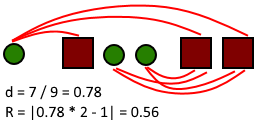
\includegraphics[scale=2]{numeric.png}
    \end{center}
    \end{itemize}
    }
 
 
    \column{0.5}
    \block{Ideas}{
    \begin{itemize}
    \item
    We could pick a smaller subset of more relevant columns
    \item
    We need to find a way to estimate a relevance of columns
    \item
    We also need the relevance measures of categorical and numeric columns to be comparable
    \item
    Maximizing MCC roughly corresponds to maximizing accuracy in a balanced dataset
    \item
    For performance reasons it's a good idea to use undersampling, the patterns in
    overrepresented outcome will likely remain detectable
    \end{itemize}
    }
    
    \block{Categorical Relevance Measure}{
    \begin{itemize}
    \item
    Assign success with weight $w_s$ and failure with weight $w_f$
    \item
    If a category has $a$ successful products and $b$ failures, its proportional failure is:
    \[
    	p = b \cdot w_f / (a \cdot w_s + b \cdot w_f)
    \]
    \item
    Proportional failure can be used as a numeric value of category. The relevance measure is:
    \[
    	r = |p \cdot 2 - 1|
    \]
    \begin{center}
    \includegraphics[scale=2]{categorical.png}
    \end{center}
    \end{itemize}
    }
    
    \block{Modeling}{
    \begin{itemize}
    \item
    Even with subsampling, the dataset sizes turned out too much for R to handle, so I had to turn to python
    \item
    I some tried simple neural network architectures in Python using Keras
    \item
    In the end the highest validation accuracy I managed was around 64\%, which is not high considering there were only 2 classes
    \item
    In the end I suspect there is not much much more I could have done with models. Probably even more effort is needed in preprocessing and feature extraction
    \end{itemize}
    }
    
    
\end{columns}
 
\end{frame}
\end{document}